\documentclass[12pt,fleqn]{article}
\setlength{\parindent}{0pt}
\usepackage{graphicx}
\usepackage{listings}
\usepackage[latin5]{inputenc}
\setlength{\parskip}{8pt}
\setlength{\parsep}{0pt}
\setlength{\headsep}{0pt}
\setlength{\topskip}{0pt}
\setlength{\topmargin}{0pt}
\setlength{\topsep}{0pt}
\setlength{\partopsep}{0pt}
\setlength{\mathindent}{0cm}

\begin{document}
MIT OCW Hesapsal Bilim 18.085 Ders 5

Onceki derste $-u'' = \delta(x-a)$ denklemini cozmustuk. Ayriksal olarak bu
denklem sol tarafta matris $-K$, sag tarafta ise noktasal agirligi tek
hucre icinde 1 olan bir vektore tekabul edecektir. K baglaminda 1 -2 1
formu, -1 2 -1 haline gelir, $u$ vektoru onceki gibi, sag tarafta ise
ayriksal delta fonksiyonu. Agirligin 2. hucrede oldugu ornek alttadir. 

\[  
\left[\begin{array}{cccc}
2 & -1 & 0 & 0 \\
-1 & 2 & -1 & 0 \\
0 & -1 & 2 & -1 \\
0 & 0 & -1 & 2 
\end{array}\right]
\left[\begin{array}{c}
u_1 \\
u_2 \\
u_3 \\
u_4
\end{array}\right]
=
\left[\begin{array}{c}
0 \\
1 \\
0 \\
0
\end{array}\right]
\]

Ortaya ilginc bir durum cikti: sag taraftaki matrise bakarsak, agirlik
2. hucrede ve orasi 1. Eger 3. olsaydi 3. hucre 1 olurdu, vs. Tum bu
vektorleri yanyana koysak, birim matrisini elde etmez miyiz? Evet. O zaman
bir kolaylik ortaya cikti. Agirlik $j$ uzerinde ise o vektoru $\delta_j$
ile temsil edersek, 

\[ Ku = \delta_j \]

$\delta_j$ yerine $I$ kullanirsak, ve $u$ vektoru yerine $U$ kullanirsak,

\[ KK^{-1}U = I \cdot K^{-1}\]

\[ U = K^{-1} \]

olacaktir. $U$ icinde her turlu $j$ olasiligi icin bir cozum iceriyor. Eger
$j=2$ olasiliginin cozumunu gormek istiyorsak o zaman $K^{-1}$ matrisinin
yani $U$'nun 2. kolonuna bakmak yeterli.

Peki, eger yuk tek bir nokta yerine ``tum'' noktalarda olsaydi ne yapardik?
Tum noktalardaki yuk esitligin sag tarafinin tamamen 1 olmasi demektir. O
zaman bir baska numara yaparak, tamamen 1 iceren bu vektoru ayri ayri
$\delta_j$'ler ``toplami'' olarak gorebiliriz, mesela

\[ 
\left[\begin{array}{c} 1 \\ 0 \\ 0 \\ 0  \end{array} \right] +
\left[\begin{array}{c} 0 \\ 1 \\ 0 \\ 0  \end{array} \right] +
\left[\begin{array}{c} 0 \\ 0 \\ 1 \\ 0  \end{array} \right] +
\left[\begin{array}{c} 0 \\ 0 \\ 0 \\ 1  \end{array} \right] = 
\left[\begin{array}{c} 1 \\ 1 \\ 1 \\ 1  \end{array} \right] 
 \]

Bu ne demektir? Esitligin sag tarafinin ``girdi'' olarak gorulebildigini de
biliyoruz. Lineer bir sistemde girdiler toplanirsa, mumkun tum ciktilar da
toplanir. Ustteki $K^{-1}$'in kolonlari da bu mumkun tum ciktilari zaten
verdigine gore tek yapmamiz gereken bu kolonlari birbiriyle toplamaktir. 

Green'in Fonksiyonu

$-u''$'ya esit olarak bir noktasal agirlik (point load) yani delta
fonksiyonu varsa cikan sonuc Green'in fonksiyonu olarak bilinir ve
bu fonksiyon $G(x,a)$ olarak ta gosterilebilir, cunku Green'in fonksiyonu hem
$x$'e hem $a$'ya baglidir. Ayriksal, surekli (continuous) baglaminda ise
Green'in fonksiyonu ustte gosterilen matris tersi isleminin surekli hali
olarak dusunulebilir. 

Ozdegerler ve Ozvektorler (Eigenvalues and Eigenvectors)

Ozdegerler $Ay = \lambda y$ formunda ortaya cikarlar. Eger bir problemde bu
formu bulabilirsek, cozum icin muthis kolaylik saglayan bir
kavramdirlar. Ozdegerler $\lambda$ icinde, ozvektorler $y$ icinde bulunur. 

Bu kavram hakkinda anlayis gelistirelim. Mesela elimizde bir $v$ vektoru
var, ve $A$ matrisi ile carpiliyor. Sonuc yine bir vektor olacak, bu vektor
$Av$ vektoru. 

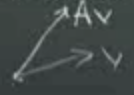
\includegraphics[height=2cm]{5_2.png}

Eger o vektor yukaridaki gibiyse, $v$ bir ozvektor {\em degil}
demektir. Niye? Cunku ozvektorler ozel vektorlerdir (her $A$ icin) , oyle
degerlere sahiptirler ki $A$ ile carpilinca, cizgisel {\em yonleri}
degismez (ama boylari degisebilir). Diyelim ki elimizde bir $y$ var,

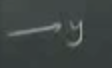
\includegraphics[height=1cm]{5_3.png}

$Ay$ alttaki gibi olabilir

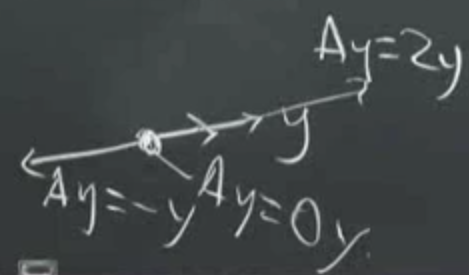
\includegraphics[height=2cm]{5_4.png}

$2y$ olabilir, ters yonde buyuyebilir, sifir haline de gelebilir, vs. Fakat
muhakkak ayni cizgi uzerinde kalir, $\lambda$ degeri de 2, sifir, vs gibi
buyumenin, kuculmenin ne kadar oldugunu belirten degerler olacaktir. Fakat,
tekrarlamak gerekirse, ozvektorler nadirdirler zaten tarif edildigi sekilde
davranan bir vektorun az rastlanan bir sey olmasi normal olmalidir.

Bunun faydasi, degeri nedir? Ozvektor bize oyle bir yon saglar ki o yonde
$A$ bir sayi gibi davranir. $A$, $y$ vektorunu ``degistiren'', onu
transform eden bir fonksiyondur bir bakima, ve bu fonksiyon ne kadar
cetrefil olursa olsun belli bir ``ozel'' yonde sadece sayi etkisi
yapmaktadir. Mesela

\[ \frac{du}{dt} = Au \]

diyelim ki $u$ 1000 boyutunda bir vektor, $A$ 1000 x 1000 boyutunda bir
matris. Denklem cok buyuk, ama diyelim ki biz bu $A$ icin oyle bir ozvektor
ve ozdeger $u$ biliyoruz ki (eger bu degerler problem icinde mantikli
degerler de iseler) o zaman sunu da biliyoruz ki cozum o yonde baslarsa o
yonde kalir.

O zaman elimizde bir skalar var demektir (cunku $A$ yonde tek sayi etkisi
yapiyor) yani ustteki diferansiyel denklem $u' = Au$ yerine $u' = \lambda
u$ haline 
gelebilir.

Bu daha basit denklemin direk analitik cozumunu biliyoruz:

\[ u = ce^{\lambda t} \]

$\lambda$ ozdeger olarak belli bir yondeki buyume, kuculmeyi gosteriyorsa,
ustteki formul icinde de benzer anlami tasir: Arti $\lambda$ ustel deger
uzerinden ona oranli bir buyumeyi, eksi olani o oranda bir kuculmeyi
gosterir. Guzel. Kavramlar birbiriyle baglantili cikiyor, demek ki dogru
yoldayiz.

Diger kullanimlar? Temel denklemi tekrar yazalim. 

\[ Ay = \lambda y \]

Soru su: $A^2$ icin oyle bir vektor ariyorum ki $A$ ile iki kez carpinca
yon degistirmiyor. Cevap, yine ozvektor $y$. Cunku $y$'yi $A$ ile carpinca
$\lambda y$ cikiyor, yon hala degismedi, o zaman bir daha carparsak, yon
hala ayni kalir, bu sefer sonuc $\lambda^2y$.

\[ A^2 = \lambda^2 y \]

Ozvektorler diferansiyel denklemler icin, bir matrisin ustel degerlerini
hesaplamak icin cok faydalidirlar. Bir matrisin pivotlari sabit konum
(steady-state) problemini incelerken de elimizdeki onemli sayilardir
onlar. Hareket halindeki bir maddeyi incelerken yardimci olurlar, salinimi
(oscillate), buyuyen, kuculen seyleri incelemekte faydalidirlar.

Eger $\lambda$ kompleks bir sayi olsaydi? O zaman $\lambda$'nin reel
bolumune bakardik, $< 0$ ise, stabil kuculme (decay), buyuk ise stabil
olmayan buyume (growth) olurdu. Eger $e^{4it}$ gibi bir deger olsaydi, bu
pur salinim olacakti, cunku acilimi $cos(4t) + isin(4t)$ formuludur.

Diger bir soru: $k$ buyurken $A^k \to 0$ ise, yani $A$'yi surekli kendisi
ile carparken sonuc hep kuculuyorsa, bu durumu $\lambda$'ya bakarak nasil
anlayabilirim? 

$A^ky$ ise $\lambda^ky$ demektir (ustte gorduk), o zaman $A^ky$'nin nasil
davranacagini $\lambda^ky$'a bakarak anlayabilirim. $\lambda^ky$ ne zaman
sifira gider? Cevap: $\lambda < 1$ oldugu zaman.

Kompleks $\lambda$'li Reel Matris

Diyelim ki elimizde bir vektoru 90 derece dondurebilen bir $A$ matrisi
var. 

\[ 
A = 
\left[
\begin{array}{rr}
0 & -1 \\
1 & 0
\end{array}
\right]
 \]

Bu matrisin reel ozdegerleri olamaz, cunku bu matrisin uygulanip yonu
degismeyen hicbir ``reel'' vektor olamaz. Gozle gorulebilen her vektor 90
derece transform edilir. Iste bu gibi orneklerde ozdeger bulmak icin
kompleks vektorler gerekir. Su vektoru deneyelim: $[1 \ \ \ i]$. 

\[ 
\left[\begin{array}{rr}
0 & -1 \\
1 & 0
\end{array}\right]
\left[\begin{array}{c}
1 \\
i
\end{array}\right]
= 
\left[\begin{array}{c}
-i \\
1
\end{array}\right]
= 
-i
\left[\begin{array}{c}
1 \\
i
\end{array}\right]
 \]

Vektor ise yaradi. Simdi ana noktaya gelelim. Ozdegerleri nasil
kullaniriz? Ve onlardan kac tane vardir? ``Iyi'' bir matris, ki bu tanima
her simetrik ve matris dahildir, eger mesela buyuklugu 1000 ise, o zaman
1000 tane farkli ozvektoru olacaktir. Simetrik matrislerde de o
ozvektorlerin hepsi reel olacaktir. Mesela:

\[ 
\left[\begin{array}{rr}
2 & -1 \\
-1 & 2
\end{array}\right]
 \]

2 x 2 boyutunda bu matriste 2 tane ozvektor bulmamiz lazim. Bu ufak bir
matris, ozvektorleri tahmin yapa yapa bulmaya ugrasabiliriz. [1 0] bir
ozvektor mu?  Carpimi yaparsak,

\[ 
\left[\begin{array}{rr}
2 & -1 \\
-1 & 2
\end{array}\right]
\left[\begin{array}{c}
1 \\
0
\end{array}\right]
=
\left[\begin{array}{r}
2 \\
-1
\end{array}\right]
 \]

Olmadi. Sagdaki vektor [1 0]'in bir kati degil. Not: Lineer cebirde kafadan
islem yapmanin yollarindan biri, [1 0] ile carparken 1 gorunce, soldaki
matrisin ``1. sol kolonunu oldugu gibi almak''. Peki [1 1]
denersem? 

\[ 
\left[\begin{array}{rr}
2 & -1 \\
-1 & 2
\end{array}\right]
\left[\begin{array}{c}
1 \\
1
\end{array}\right]
=
\left[\begin{array}{c}
1 \\
1
\end{array}\right]
 \]

Bu oldu. Ikinci ozvektor ne olabilir? [1 -1] deneyelim. 

\[ 
\left[\begin{array}{rr}
2 & -1 \\
-1 & 2
\end{array}\right]
\left[\begin{array}{r}
1 \\
-1
\end{array}\right]
=
\left[\begin{array}{r}
3 \\
-3
\end{array}\right]
 \]

Bu da oldu. O zaman $\lambda_1 = 1$, $\lambda_2 = 3$, ozvektorler [1 1] ve
[1 -1]. 

Bu ozvektorlere bana ne soyluyor? Onlara bakarak ana matris hakkinda ne
anlayabilirim? Bakalim, [1 1] ve [1 -1] birbirine ortagonal / dik
(orthagonal) vektorler. 

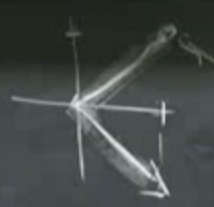
\includegraphics[height=2cm]{5_5.png}

Cebirsel olarak bu dikligi anlamak icin $y_1^Ty_2$, ya da $y_1 \cdot y_2$
hesabini yapabilirdik, diklik var ise sonuc sifir cikardi. Ozvektorlerin
dikligi baska bir sey daha soyler, simetrik matrislerin ozvektorleri
birbirine diktir, o zaman sadece ozvektorlere bakarak ana matrisin simetrik
oldugunu anlayabilirdik.

Soylemeye calistigimiz ozdeger ve ozvektorler matrisleri incelemenin,
onlarin ``icine bakmanin'' yollarindan bir tanesidir. 

Peki ustteki simetrik olmayan matrise donersek

\[ 
\left[
\begin{array}{rr}
0 & -1 \\
1 & 0
\end{array}
\right]
 \]

Bu matrisin ozvektorleri kompleks cikmisti, ki bu durum simetrik olmayan
matrislerin bir ozelligidir. Simetrik matrisleri bu sebeple tercih ederiz,
ozvektorleri reel, birbirine dik.

Ozdegerler uzerinde guzel iki tane faydali kontrol mekanizmasi: $\lambda_1
= 1$, 
$\lambda_2 = 3$ buldugumuz ornekte iki ozdeger toplami nedir? 4. Ana
matrisin caprazindaki degerleri toplarsak (buna matrisin ``izi'' -trace-
adi da verilir)

\[ 
\left[\begin{array}{rr}
2 & -1 \\
-1 & 2
\end{array}\right]
 \]

Sonuc yine 4. Bu iki toplam her zaman esit cikmalidir. Bir numara: bir
tanesi haric tum ozdegerleri bulduksak matrisi izini kullanarak sonuncu
ozdegeri hizla bulabiliriz, cunku capraz toplamindan diger ozdeger
toplamini cikartiriz, kalan sonuncu ozdeger olmalidir.

Bir kontrol daha. Ozdegerleri birbiriyle carparsam sonuc 3 cikar. Ana
matrisin determinantini alirsam sonuc yine 3 cikar. Bu iki kontrol
teknigini, ispatini gostermeden, burada vermis olalim. 

Kullanima gelelim: Diyelim ki elimizde icinde 1000 tane denklem iceren bir
lineer denklem sistemi var. 

\[ \frac{du}{dt} = Au \]

katsayilar sabit, baslangic noktasi $u(0)$. Ozdeger ve ozvektorler burada
nasil yardimci olabilir? Once onlari bulmamiz gerekir, 1000 tane ozvektor
var, onlari buluruz. Her $i$ icin 

\[ Ay_i = \lambda_i y_i \]

yani elimizdeki ozvektorler $y_1,..,y_{1000}$, ozdegerler
$\lambda_1,...,\lambda_{1000}$. 

Bu degerleri dif denklemi cozmek icin nasil kullanirim? 3 tane basamak
takip ederim. 

1. $u(0)$'i ozvektorlerin bir kombinasyonu olarak temsil et, yani
 $u(0) =
c_1y_1 + ... + c_{1000}y_{1000}$. 

2. $e^{\lambda_1t}$'yi $c_1$ ile carp, yani $c_1$'i onun buyumesi ile
carp, genel olarak $e^{\lambda_it}$'yi $c_i$ ile carp. 

3. Topla: $c_1e^{\lambda_1t}y_1 + .. + c_{1000}e^{\lambda_{1000}
  t}y_{1000}$. 

Not: Bunun niye islediginin ispati icin Lineer Cebir Ders 23'e bakilabilir.

Not: Konuyla ilgili bir problem bu notlarin en altinda.

Tabii bunu islemesi icin $u(0)$'in ozvektorlere, ozdegerlere gore
parcalanmasi gerekir, ayrica tum ozvektorlerin bulunabiliyor olmasi
gerekir. Problemimiz bize simetrik bir matris sagliyorsa sorun olmaz, ama
bazi problemlerde matris ``defolu'' olabilir, bazi ozvektorler
birbirlerinin icine girerler (collapse) ve elde yeteri kadar ozvektor
olmaz. Yani cozmeye calistigimiz probleme gore bu teknigi kullanabilir ya
da kullanamayabiliriz. 

Not: Ozvektorlerin birbirine yakin, hatta esit olma problemi ODE'lerdeki
kritik amortisorlu (critically damped) kosulda koklerin birbirine esit
cikmasiyla ayni durum (MIT OCW ODE Ders 9). Orada yeni bir cozum
``yaratmak'' icin $e^{-at}$ ile $t$'yi carpmistik. Burada da ozdegerleri
aslinda kokler olarak gorebiliriz, eger iki ozdeger esit ise, elimde sadece
bir tane ozvektor olma riski de yuksek demektir. O zaman yeni bir cozum
yaratmak icin ODE dunyasindakine benzer bir numara kullanirim, $te^{\lambda
  t}$ 
hesabini yapabilirim. 

Ek Aciklamalar

$u(0)$'i $A$'nin ozvektor lineer kombinasyonu olarak temsil edilirse,
sonucun $c_1e^{\lambda_1t}y_1 + .. + c_ne^{\lambda_n t}y_n$ seklinde
olabilecegini nereden biliyoruz?  Cunku $du/dt = Au$ ve $Au = \lambda u$
lineer denklemler. Bir sonraki adim icin $u(0)$ degistirildiginde, bu
lineer bir sekilde, $A$ uzerinden olacak, ve $A$'ya ``girdi'' olarak
verilen vektorler eger ozdegerlerin kombinasyonu ise, bu kombinasyon cikisa
da aynen, verildigi sekilde yansiyacak.

Bolum 1.5 Ornek 4 (Kitaptan)

Diyelim ki vektorel formdaki bir $u(t)$ denklemi ABD'de Missisipi nehrinin
dogusu ve batisinda $t$ anindaki nufusu temsil ediyor. Soyle:

\[ u(t+1) = Au(t) \]

Bu vektorel $u(t)$'yi bilesenleriyle soyle aciklayalim

\[ 
\left[\begin{array}{r}
t+1 \textrm{ aninda doguda olanlar } \\
t+1 \textrm{ aninda batida olanlar } 
\end{array}\right]
=
\left[\begin{array}{rr}
.8 & .3 \\
.2 & .7
\end{array}\right]
\left[\begin{array}{r}
t \textrm{ aninda doguda olanlar } \\
t \textrm{ aninda batida olanlar } 
\end{array}\right]
 \]

Buradaki $A$ matrisi belli bir gozleme dayanarak modelleyicinin buldugu bir
sey herhalde, problem onu bize veriyor. $A$ bir ``gecis fonksiyonu'', $t$
anindan $t+1$'e gecisi o yapiyor. Diyelim ki doguda 1 milyon insanla
basladik, 1 sene sonra ($A$ ile carpiyoruz) yeni rakamlar 800,000 ve
200,000 haline gelecektir. 

$A$ matrisi bir Markov matrisidir, Markov matrislerinin kolonlarinin ic
toplamlari her zaman 1'e esittir. Ozdeger / ozvektor baglaminda Markov
matrislerinin ilginc bir yani ozdegerlerinden birinin her zaman 1
olmasidir, yani $\lambda = 1$ muhakkak olacaktir. Iki boyutlu $A$ matrisi
durumunda bu cok ise yarar, cunku matris izine (trace) bakarak ve ondan 1
cikartarak ikinci ozdegeri hemen bulabiliriz. $A$'nin ozvektorleri de
$\lambda = 1$ icin [600,000, 400,000], $\lambda = 0.5$ icin [400,000, -400,000]
degerleridir. 

Simdi ilginc bir numara: eger baslangic degeri [1,000,000 0]'i ozvektorlerin
bir kombinasyonu olarak gosterirsek,

\[ u = [1,000,000 0] = 
a_1 \cdot [600,000, 400,000] + 
a_2 \cdot [400,000, -400,000] \]

$a_1$ ve $a_2$ 1 degerine esit. 

Soldan $A$ ile carpalim

\[ Au = 
A \ a_1 \cdot [600,000, 400,000] + 
A \ a_2 \cdot [400,000, -400,000] \]

\[ Au = 
 a_1 \ A \cdot [600,000, 400,000] + 
 a_2 \ A \cdot [400,000, -400,000] \]

\[ Au = 
a_1 \ \lambda_1 \cdot [600,000, 400,000] + 
a_2 \ \lambda_2 \cdot [400,000, -400,000] \]

$\lambda_1$ ve $\lambda_2$ nereden geldi? Ozvektorlerin tanimindan: $Ax =
\lambda x$. Ustteki 
kombinasyonda kullandiklarimiz ozvektor olduguna gore, onlarin $A$ ile
carpilmis hali onlarin tekrar ozdegerle carpilmis halini verecektir. 

Ayrica $\lambda_1=1$ olduguna gore, onu denklemde gostermeye gerek bile
yoktur (Markov matrisi iceren problemlerin bir guzel yan etkisi oldu
bu). $a_1$ ve $a_2$ zaten 1 degerine esitti, onlari da atabiliriz. Yani,

\[ Au = 
[600,000, 400,000] + 
\lambda_2 \cdot [400,000, -400,000] \]

Simdi gecis islemini birkac kere ust uste yapalim:

\[ A^2u = 
[600,000, 400,000] + 
\lambda_2^2 \cdot [400,000, -400,000] \]

\[ A^3u = 
[600,000, 400,000] + 
\lambda_2^3 \cdot [400,000, -400,000] \]

...

Boyle devam edecek. $\lambda_2=1/2$ olduguna gore, ve bu deger 1'den kucuk
oldugu icin $n$ buyudukce $\lambda_2^n$ cok kucuk bir sayi haline gelir, ve
sifira yaklasir. Yani ustteki denklemin sabit konum (steady-state)
cozumu [600,000, 400,000] degeridir.

Ornek Problem

\[ 
\frac{du}{dt} = Au
 \]

problemini cozdugumuzu farzedelim, ki $u(t)$ soyle tanimli

\[ 
u(t) =
\left[\begin{array}{r}
y(t) \\
z(t)
\end{array}\right]
 \]

Ayri ayri

\[ dy/dt = 2y - z \]

\[ dz/dt = -y + 2z \]

Matris formunda

\[ 
\frac{d}{dt}
\left[\begin{array}{r}
y \\
z
\end{array}\right]=
\left[\begin{array}{rr}
2 & -1 \\
-1 & 2
\end{array}\right]
\left[\begin{array}{r}
y \\
z
\end{array}\right]
 \]

ki yukaridaki 2x2 matris $A$ matrisi olacak. Lineer Cebir Ders 23'te
goruldugu gibi bu problemin cozumu 

\[ u = S e^{\Lambda t} S^{-1} u(0) \]

Hesapsal Bilim ders kitabi sayfa 53'te bu problemin sadece 

\[ u = S e^{\Lambda t} v(0) \]

noktasina kadar gelinip birakildigi bir bolum var, bu bolumun sonucunu
ustteki $u$ formulune gore yineden turetelim. $v(0) = [C \ \ D]$ seklinde
bir vektor tanimlayalim, bunlari baslangic degerlerinin ozvektorleri nasil
kombine ettigini gosteriyor. $A$ matrisinin ozdegerleri $\lambda_1=1$ ve
$\lambda_2=3$, ona tekabul eden ozvektorler [1 1] ve [1 -1]. O zaman

\[ 
u(t) =
\left[\begin{array}{rr}
1 & 1 \\
1 & -1
\end{array}\right]
\left[\begin{array}{rr}
e^{\lambda_1 t} & \\
& e^{\lambda_2 t} 
\end{array}\right]
\left[\begin{array}{r}
C \\
D
\end{array}\right]
= 
\left[\begin{array}{r}
y(t) \\
z(t)
\end{array}\right]
 \]

Bu carpimi ayri ayri yapinca cozumun kitapta gosterildigi gibi

\[  
\left[\begin{array}{r}
y(t) \\
z(t)
\end{array}\right]
=
\left[\begin{array}{r}
Ce^t + De^{3t} \\
Ce^t - De^{3t} 
\end{array}\right]
\]

olarak ciktigini gorecegiz. 

\end{document}
